\documentclass[11pt, a4paper]{article}

%===============================================================================
% PACKAGES
%===============================================================================
\usepackage[utf8]{inputenc}
\usepackage[T1]{fontenc}
\usepackage{amsmath}              % For mathematical formulas
\usepackage[margin=0.8in]{geometry} % For setting page margins
\usepackage{graphicx}             % To include graphics
\usepackage{hyperref}             % For clickable links
\usepackage{xcolor}               % For colors
\usepackage{amssymb}              % For symbols like arrows
\usepackage{fancyvrb}             % For the pseudocode box
\usepackage{float}                % For improved figure placement control

%===============================================================================
% DOCUMENT & HYPERLINK SETUP
%===============================================================================
\hypersetup{
    colorlinks=true,
    linkcolor=blue,
    filecolor=magenta,      
    urlcolor=blue,
    pdftitle={Q-Learning Gridworld Report},
    pdfauthor={Jeevan Hebbal Manjunath},
}

%===============================================================================
% TITLE
%===============================================================================
\title{\textbf{Teaching an Agent to Navigate a Risky World: \\ A Q-Learning Adventure}}
\author{Jeevan Hebbal Manjunath}
\date{\today}

%===============================================================================
% DOCUMENT START
%===============================================================================
\begin{document}

\maketitle

\begin{abstract}
In this report, we explore how a simple agent can learn complex, intelligent behavior through pure trial and error. We apply the Q-learning algorithm to a classic gridworld problem, a world filled with rewards, penalties, and unpredictable movement. Through a comprehensive analysis of the agent's learning process, hyperparameter tuning, and final strategies in both standard and high-risk environments, we demonstrate its remarkable ability to adapt its behavior in response to potential danger.
\end{abstract}

\hrule
\vspace{1em}

%===============================================================================
\section{The Challenge: A Risky Gridworld}
%===============================================================================
Imagine a robot trying to find its way through a maze. The floor is slippery, so moving forward might cause it to slide sideways. The maze has a goal with a prize, but also a dangerous trap. This is exactly the challenge we've set for our learning agent.

The world is a $3 \times 4$ grid. The agent's mission is to get from the start at (1,1) to the prize at (4,3), which gives a `+1` reward. To make things harder, there's a wall at (2,2), a living penalty of `-0.04` for every move, and the agent's movement is stochastic—it only follows its intended direction 80\% of the time.

%===============================================================================
\section{Our Approach: Learning from Experience}
%===============================================================================
How can an agent learn with no initial instructions? We used Q-learning, a powerful reinforcement learning technique.

\subsection{The ``Cheat Sheet'' Analogy}
At its heart, Q-learning is like creating a ``cheat sheet'' (called a \textbf{Q-table}) for the agent. This cheat sheet has a score for every possible action in every possible square. A high score says ``This is a great move!'' while a low score says ``Avoid this!''

Initially, the agent knows nothing, so all the scores are zero. But as it explores the world, it constantly updates the cheat sheet based on the rewards and penalties it finds. The formula it uses to update the scores is:

\begin{equation}
Q(s, a) \leftarrow Q(s, a) + \alpha [r + \gamma \max_{a'} Q(s', a') - Q(s, a)]
\end{equation}

This looks complex, but it simply means: ``The new score for this move is a blend of the old score and any new information we just learned.''

\subsection{The Learning Algorithm}
The agent's training process is a continuous loop of exploring and updating its cheat sheet. To make sure it doesn't just stick to the first path it finds, we use an $\epsilon$-greedy strategy: most of the time it follows its cheat sheet, but sometimes it tries a random move, just to see what happens. This randomness (exploration) fades over time as the agent becomes more confident.

\begin{center}
\begin{BVerbatim}[frame=single, label=Algorithm Pseudocode]
Initialize the Q-table with all zeros for every state-action pair.
Set the learning parameters (alpha, gamma, epsilon).

For a large number of episodes:
    1. Place the agent at the START state.

    2. While the agent has not reached a terminal state (prize or trap):
        a. Decide whether to explore or exploit:
           --- With probability epsilon, choose a random action.
           --- Otherwise, choose the best action from the Q-table for the current state.

        b. Perform the chosen action.
        
        c. Observe the reward and the new state.
        
        d. Update the Q-table score for the action just taken using the Q-learning formula.
        
        e. Move to the new state.

    3. Slightly decrease epsilon to encourage less exploration over time.
\end{BVerbatim}
\end{center}

%===============================================================================
\section{Discussion of Findings}
%===============================================================================
The Q-learning agent successfully learned to navigate the gridworld. Analyzing its learning process and final strategies reveals key insights into how the algorithm operates and adapts.

\subsection{Comparing Standard vs. High-Risk Scenarios}
To see how the agent adapts to risk, we compared the learned policies from two different experiments: a standard run with a small penalty of -1, and a high-risk run with a massive penalty of -200.

\subsubsection{Case 1: Standard Penalty (-1)}
In the standard case, the agent learns an efficient and safe policy, shown in Figure~\ref{fig:policy_standard}. The optimal path is to move up the left side and across the top, safely avoiding the column with the penalty. This is a logical and effective strategy.

\begin{figure}[H]
    \centering
    \begin{tabular}{|c|c|c|c|}
        \hline
        $\rightarrow$ & $\rightarrow$ & $\rightarrow$ & \textbf{+1.0} \\
        \hline
        $\uparrow$ & WALL & $\uparrow$ & \textbf{-1.0} \\
        \hline
        $\uparrow$ & $\leftarrow$ & $\uparrow$ & $\leftarrow$ \\
        \hline
    \end{tabular}
    \caption{The agent's learned strategy for the standard problem (penalty = -1).}\label{fig:policy_standard}
\end{figure}

\subsubsection{Case 2: High-Risk Penalty (-200)}
When the penalty is increased to -200, the agent becomes extremely \textbf{risk-averse}, as seen in Figure~\ref{fig:policy_high_risk}. The new policy shows two key changes:
\begin{enumerate}
    \item \textbf{Strong Aversion:} Any state near the `-200` trap now has a policy that points sharply away from it. The policy in state (3,2), for example, changes from `$\uparrow$` to `$\leftarrow$`.
    
    \item \textbf{``Hunker Down'' Strategy:} In the bottom-right corner (4,1), the agent's policy is to move `$\downarrow$`, causing it to stay put. It has learned that doing nothing is safer than risking a move that might stochastically slip toward danger.
\end{enumerate}

This comparison makes it clear that the agent doesn't just learn a single path; it learns the true value of its actions and adapts its strategy to become more cautious as the environment becomes more dangerous.

\begin{figure}[H]
    \centering
    \begin{tabular}{|c|c|c|c|}
        \hline
        $\rightarrow$ & $\rightarrow$ & $\rightarrow$ & \textbf{+1.0} \\
        \hline
        $\uparrow$ & WALL & $\leftarrow$ & \textbf{-200.0} \\
        \hline
        $\uparrow$ & $\leftarrow$ & $\leftarrow$ & $\downarrow$ \\
        \hline
    \end{tabular}
    \caption{The agent's highly cautious strategy with a -200 penalty.}\label{fig:policy_high_risk}
\end{figure}
\subsection{The Crucial Role of Hyperparameters}
The agent's learning effectiveness is highly dependent on tuning its core hyperparameters ($\alpha, \gamma, \epsilon$). Figure~\ref{fig:hyperparameter_summary} provides a high-level conceptual overview of their effects.

\begin{itemize}
    \item \textbf{Learning Rate ($\alpha$):} Controls how \textbf{impressionable} the agent is. A high $\alpha$ leads to faster learning but can be unstable, while a low $\alpha$ is stable but slow.
    
    \item \textbf{Discount Factor ($\gamma$):} Controls how \textbf{farsighted} the agent is. A high $\gamma$ is essential for prioritizing long-term rewards like the `+1` prize over short-term penalties.
    
    \item \textbf{Exploration Schedule ($\epsilon$ decay):} A \textbf{decaying schedule} is best. The agent starts with high randomness to explore, then gradually reduces it to exploit the optimal path it has found.
\end{itemize}

\begin{figure}[H]
    \centering
    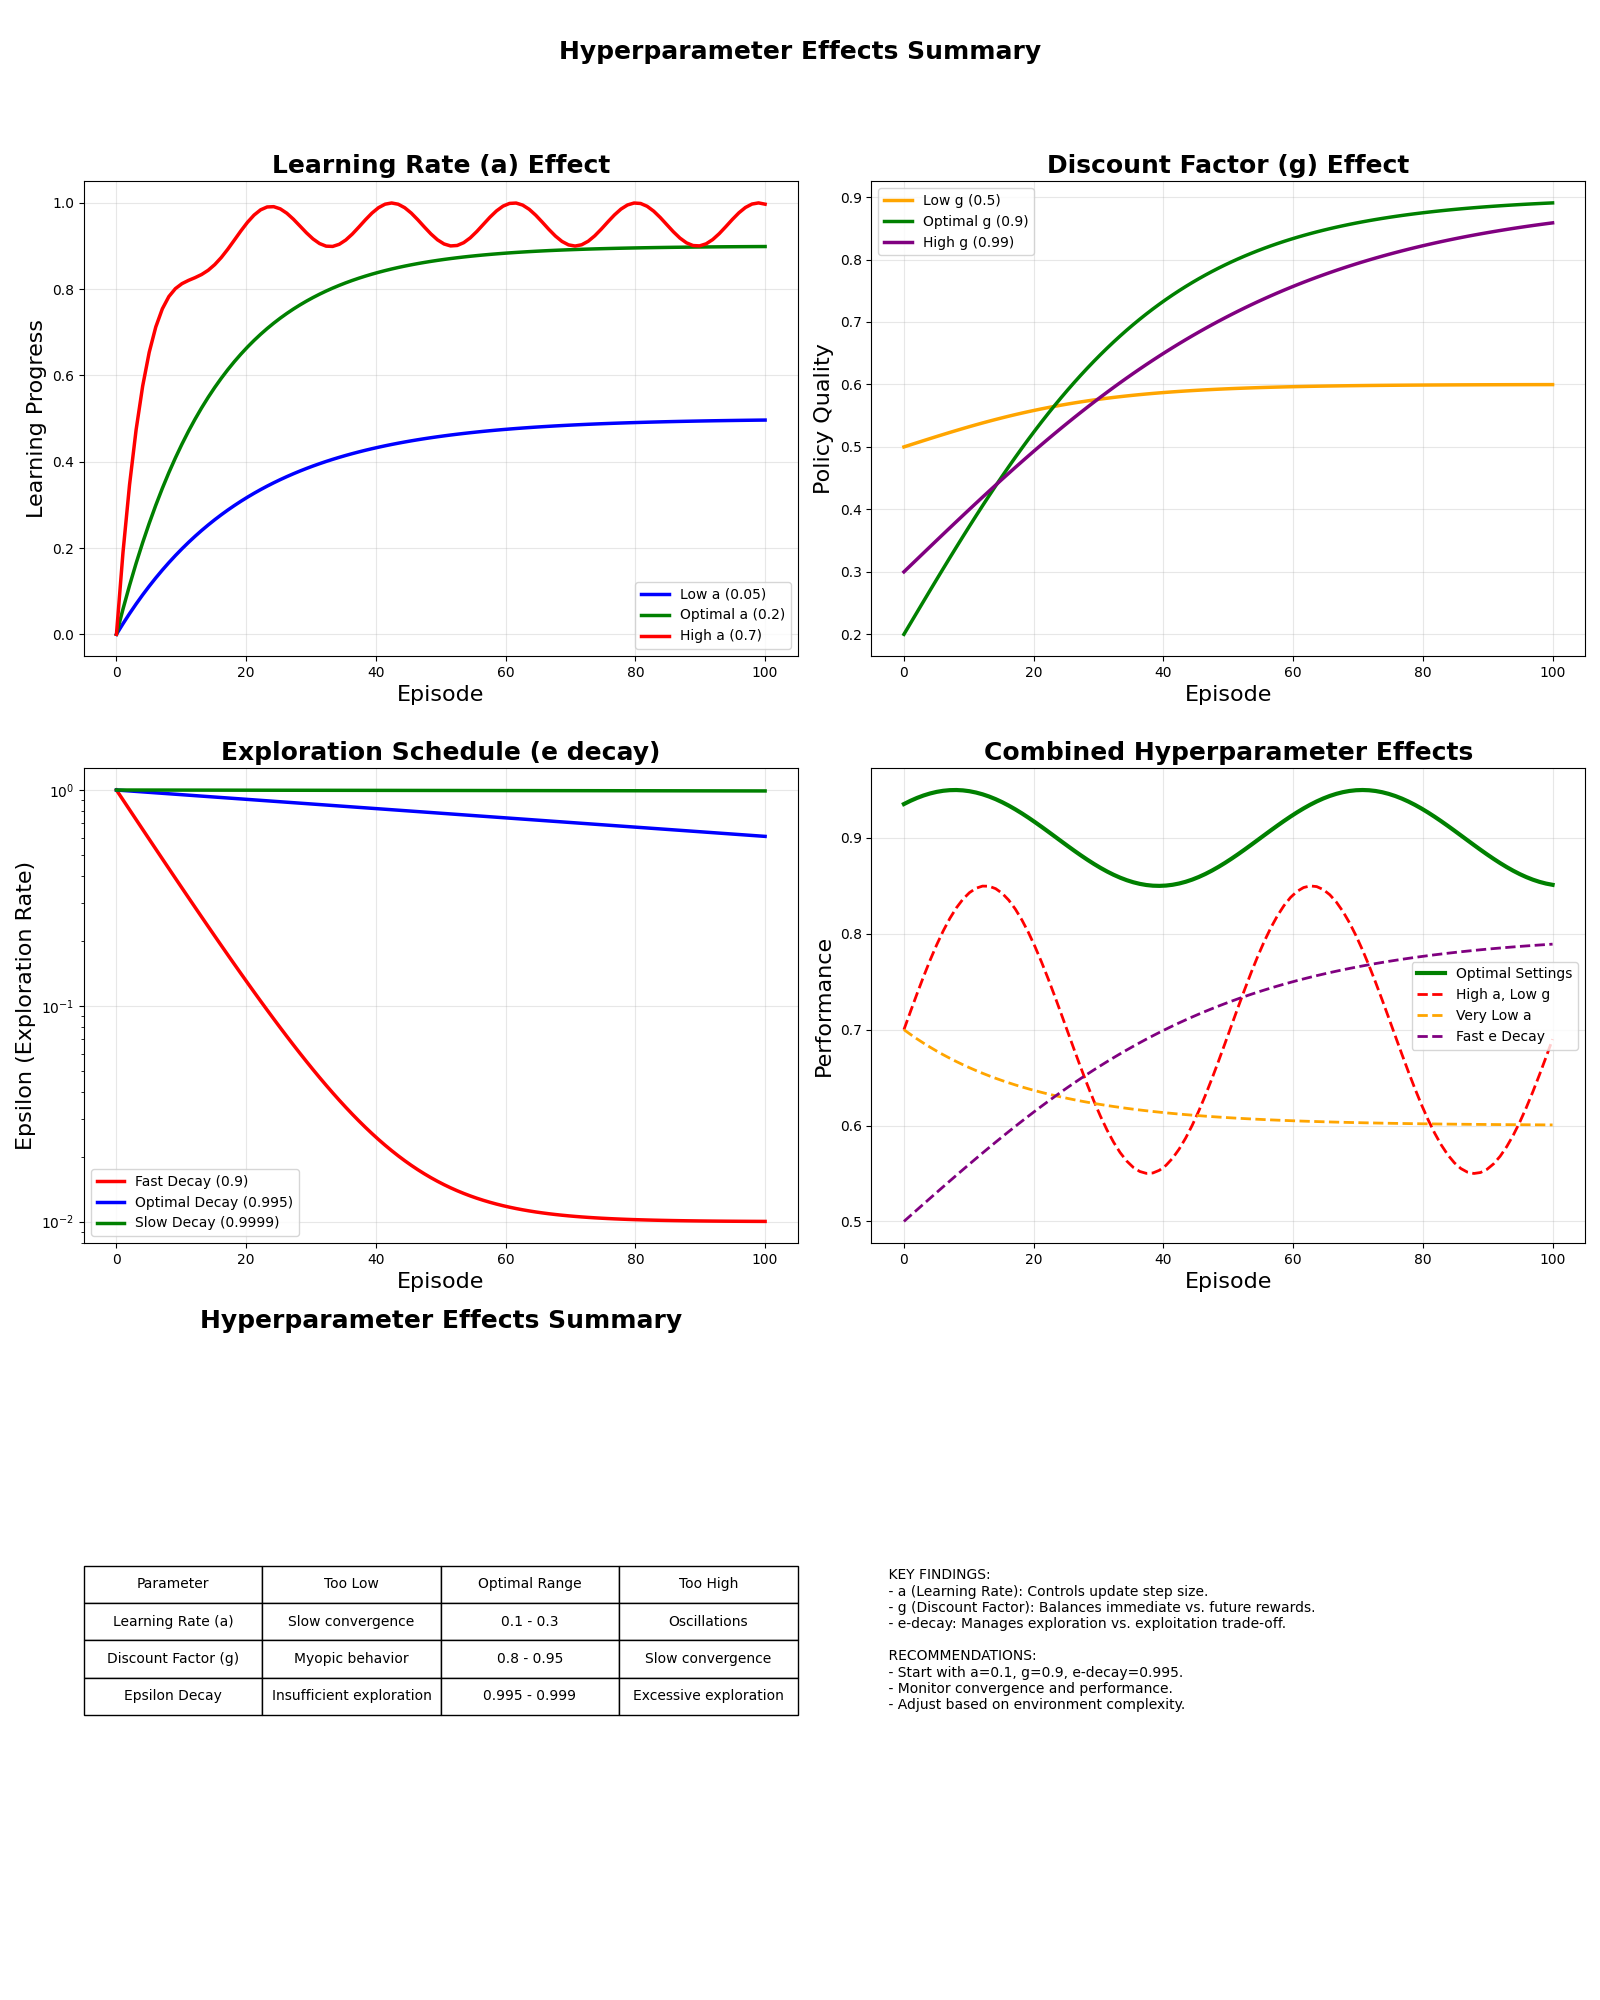
\includegraphics[width=0.9\textwidth]{images/hyperparameter_effects_summary.png}
    \caption{A conceptual summary of how learning rate ($\alpha$), discount factor ($\gamma$), and the exploration schedule ($\epsilon$) impact Q-learning performance, with a table summarizing optimal ranges.}\label{fig:hyperparameter_summary}
\end{figure}

A more detailed, data-driven analysis is presented in the following figures. This comprehensive plot reveals several key trade-offs:
\begin{itemize}
    \item Figure~\ref{fig:hyperparameter_alpha} shows that an intermediate learning rate ($\alpha \approx 0.1-0.3$) provides the best balance between convergence speed and stability. Very high values lead to erratic performance.
    \item Figure~\ref{fig:hyperparameter_gamma} confirms that a high discount factor ($\gamma \geq 0.9$) is necessary for achieving a good policy, as it encourages long-term planning.
    \item Figure~\ref{fig:hyperparameter_epsilon} illustrates different exploration schedules. A moderate decay rate (e.g., 0.999) allows for sufficient exploration without wasting too much time on random actions.
    \item Figure~\ref{fig:hyperparameter_heatmap} visually summarizes the performance for different $\alpha$-$\gamma$ pairs, highlighting a ``sweet spot'' of high performance in the upper-right quadrant (high $\gamma$, moderate $\alpha$).
    \item Figure~\ref{fig:hyperparameter_efficiency} shows how the episode length changes as the agent learns.
\end{itemize}

\begin{figure}[H]
    \centering
    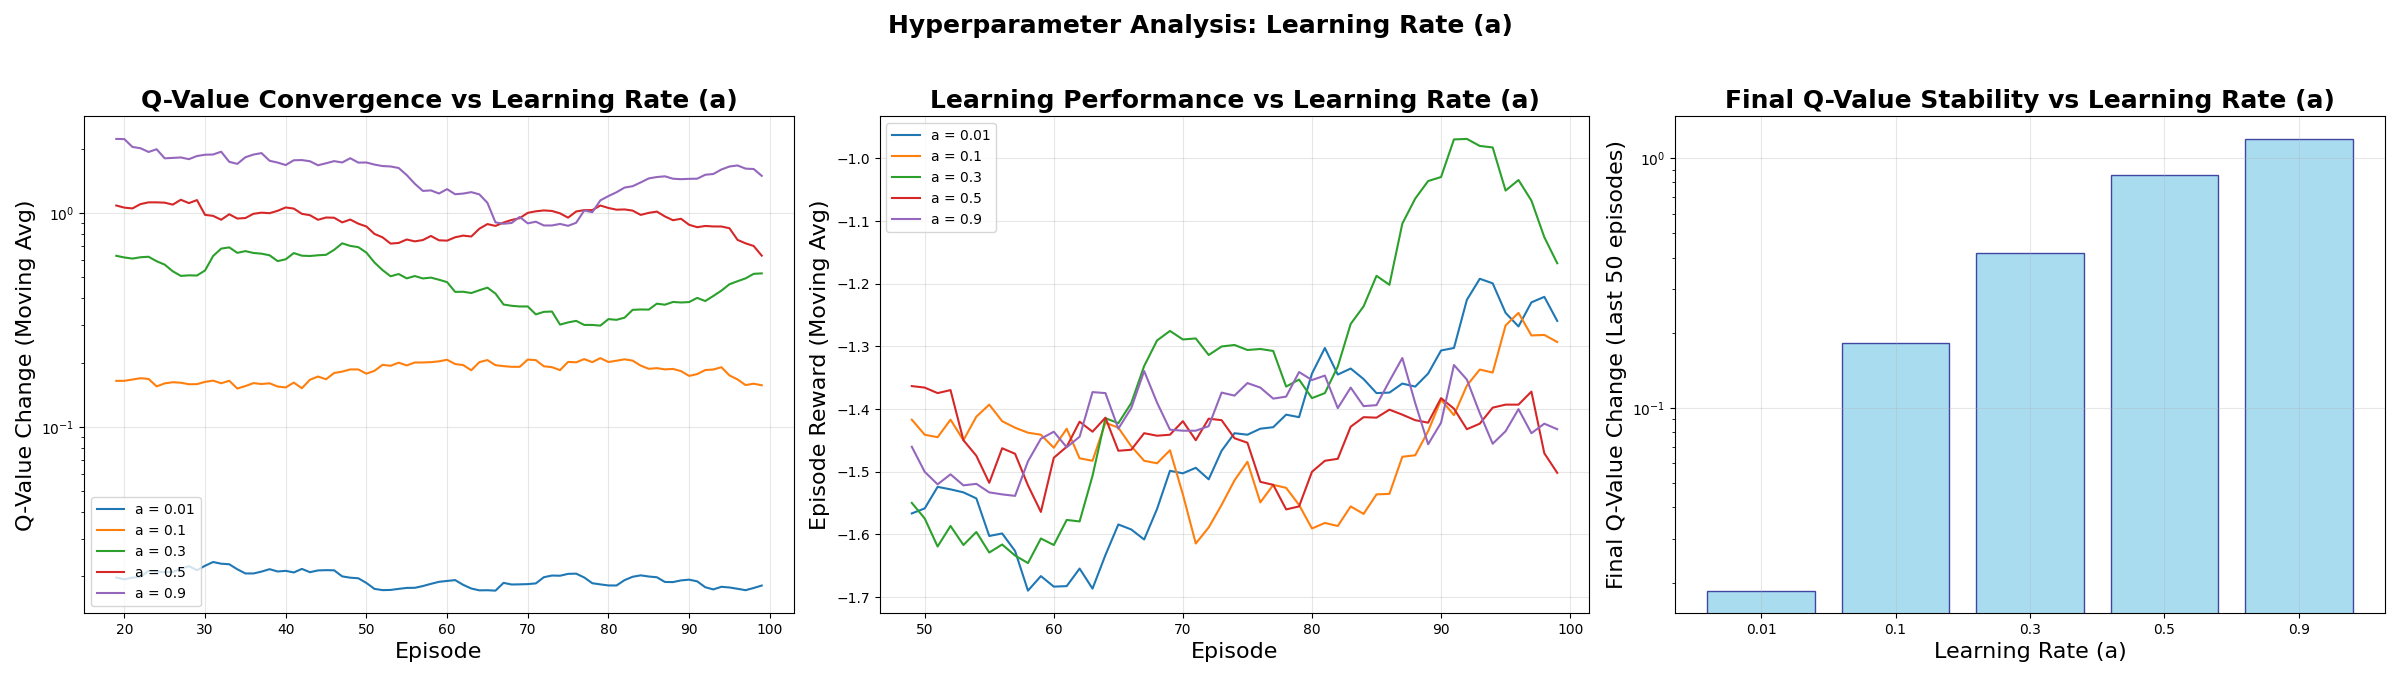
\includegraphics[width=\textwidth]{images/hyperparameter_analysis_alpha.png}
    \caption{Analysis of the Learning Rate (alpha) on Q-value convergence and learning performance.}\label{fig:hyperparameter_alpha}
\end{figure}

\begin{figure}[H]
    \centering
    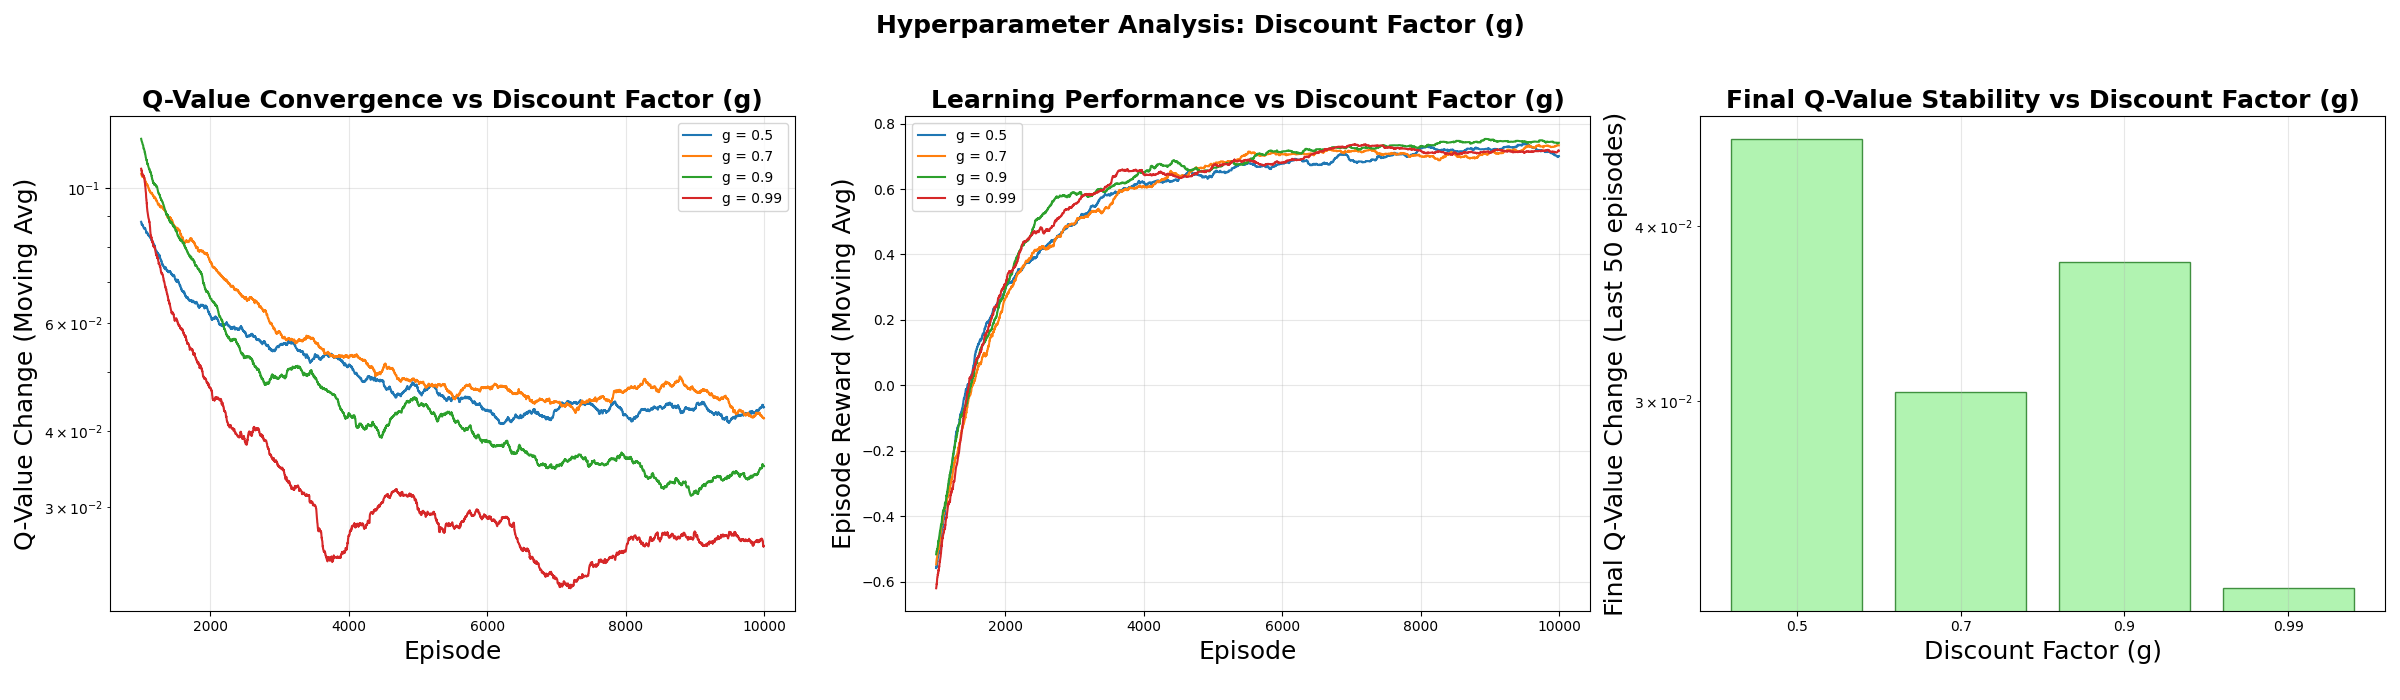
\includegraphics[width=\textwidth]{images/hyperparameter_analysis_gamma.png}
    \caption{Analysis of the Discount Factor (gamma) on Q-value convergence and learning performance.}\label{fig:hyperparameter_gamma}
\end{figure}

\begin{figure}[H]
    \centering
    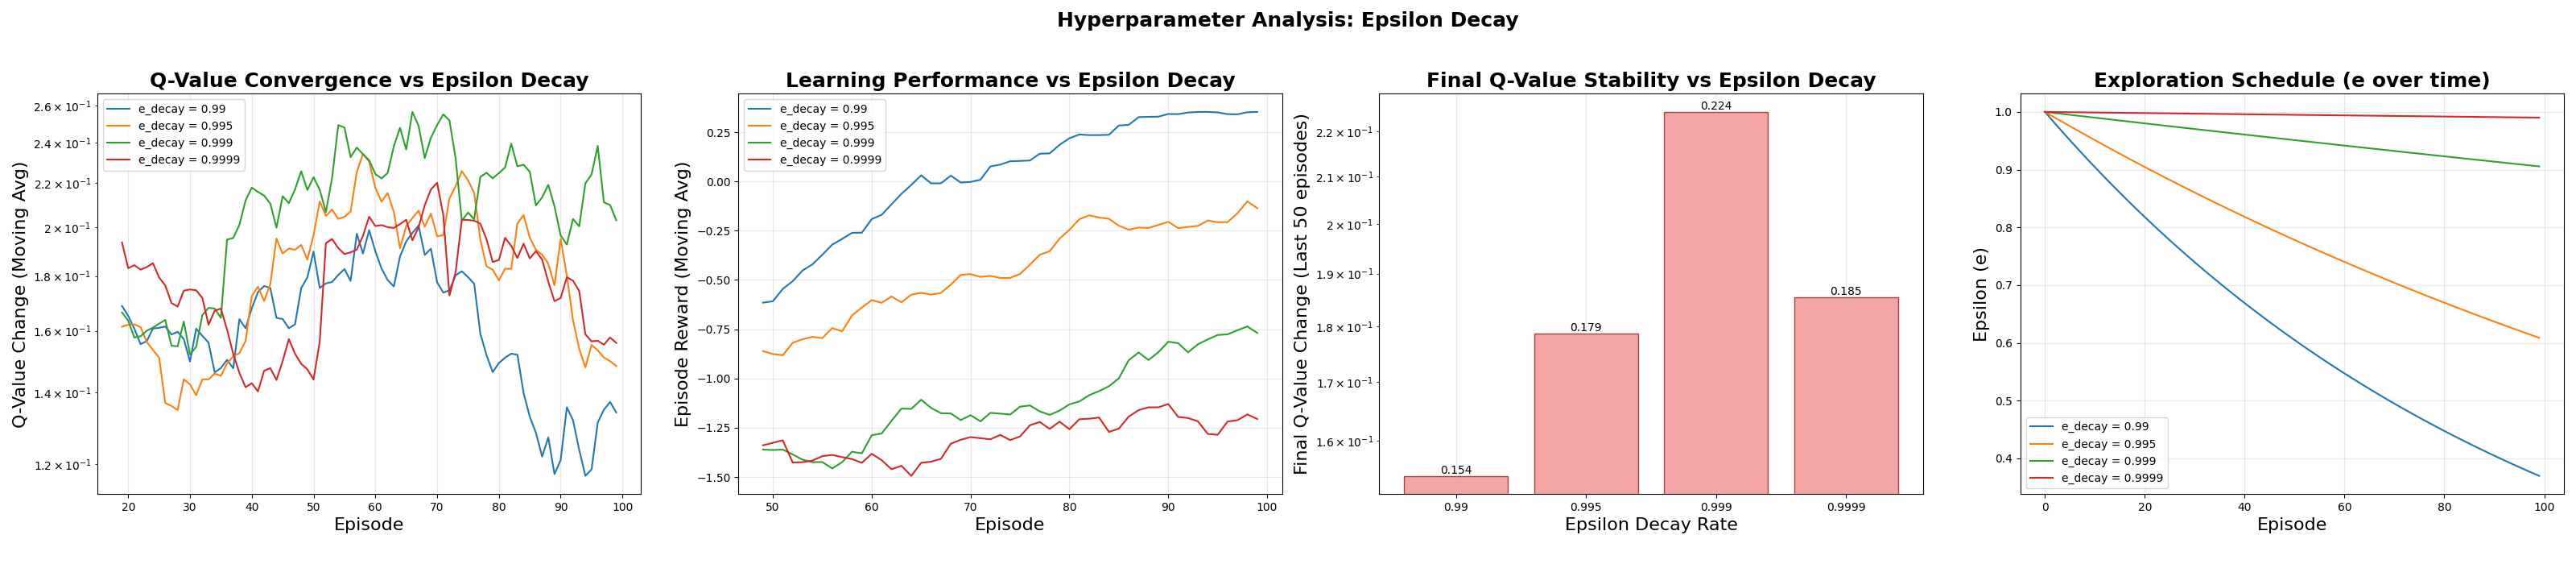
\includegraphics[width=\textwidth]{images/hyperparameter_analysis_epsilon_decay.png}
    \caption{Analysis of the Epsilon Decay on Q-value convergence and learning performance.}\label{fig:hyperparameter_epsilon}
\end{figure}

\begin{figure}[H]
    \centering
    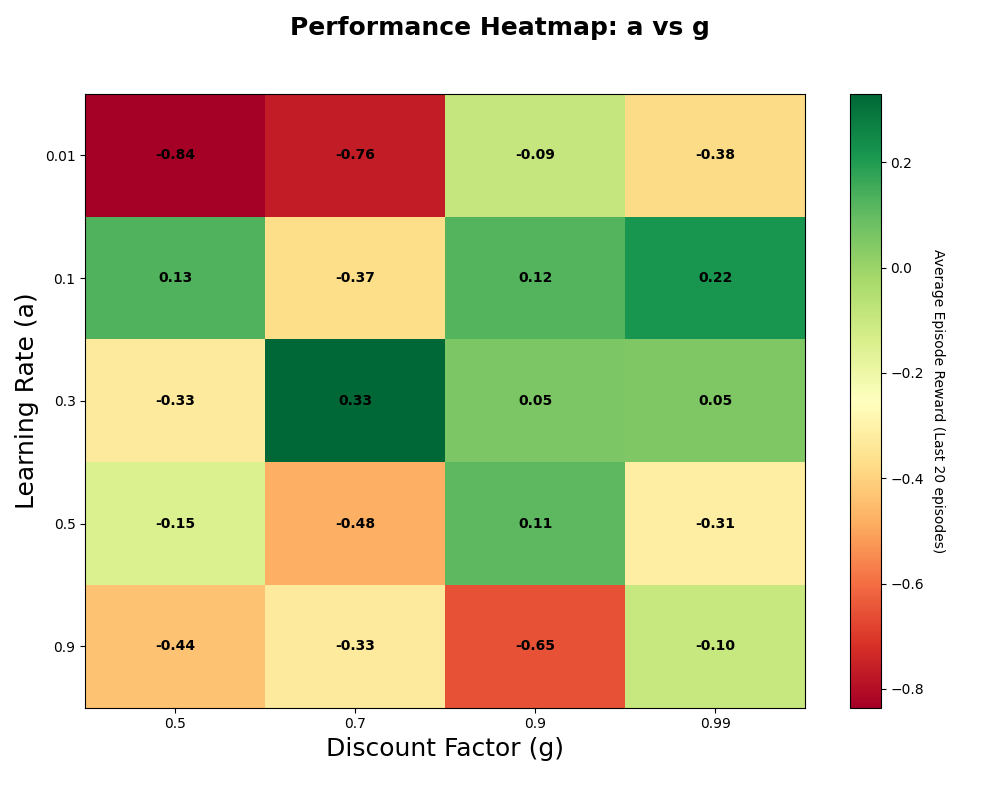
\includegraphics[width=0.9\textwidth]{images/hyperparameter_heatmap.png}
    \caption{A heatmap showing the performance of different combinations of learning rate ($\alpha$) and discount factor ($\gamma$).}\label{fig:hyperparameter_heatmap}
\end{figure}

\begin{figure}[H]
    \centering
    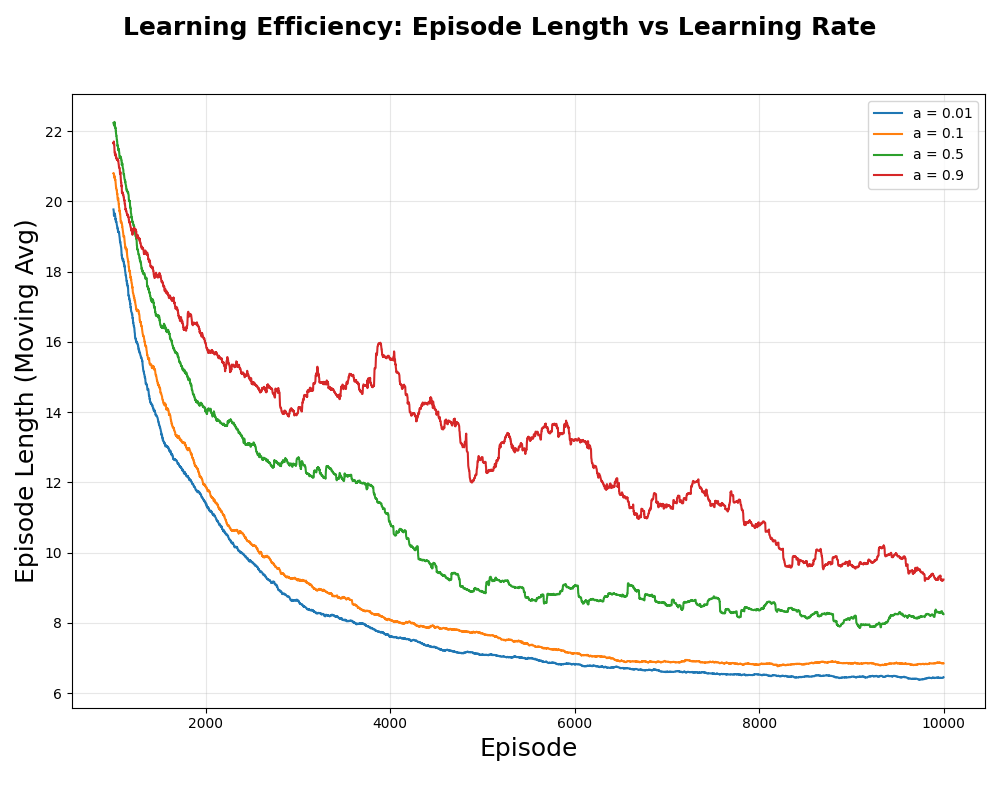
\includegraphics[width=0.9\textwidth]{images/hyperparameter_efficiency.png}
    \caption{Learning efficiency for different learning rates.}\label{fig:hyperparameter_efficiency}
\end{figure}

\subsection{Understanding Convergence: Policy vs. Q-Values}
An important observation is that the agent's \textbf{policy converges much earlier than its Q-values}. The policy—what the agent decides to do—only depends on which action has the highest Q-value in a state. This relative ordering can stabilize long before the Q-values themselves stop changing numerically.

As shown in Figure~\ref{fig:convergence}, the number of policy changes (bottom plot) drops to zero after about 40 episodes, meaning the agent has settled on a final strategy. However, the total change in Q-values (top plot) continues to fluctuate for the entire training run, as the agent fine-tunes its ``cheat sheet'' scores. This demonstrates that a stable, optimal policy can be achieved well before the underlying value function has fully converged.

\begin{figure}[H]
    \centering
    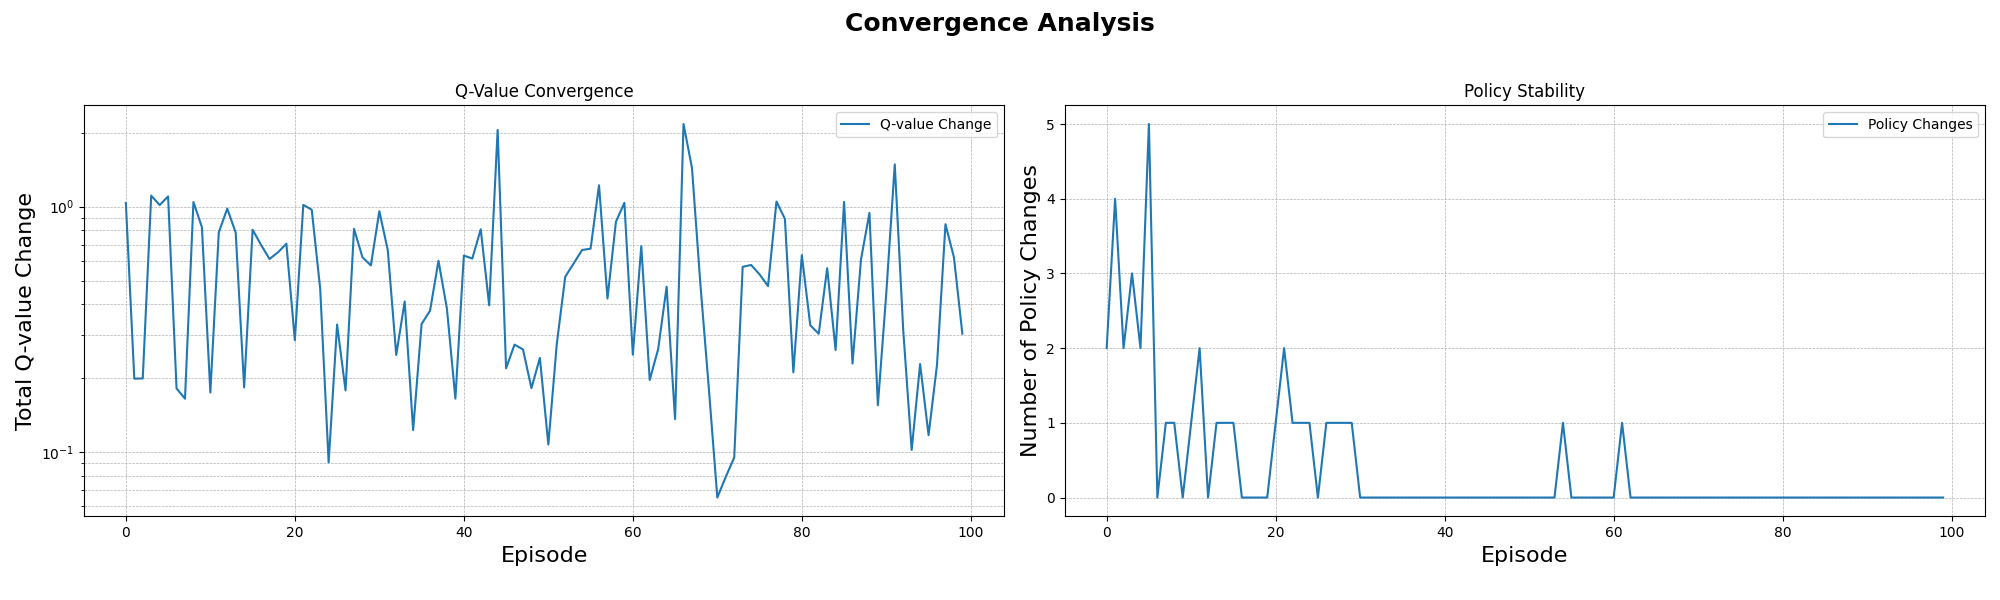
\includegraphics[width=0.8\textwidth]{images/convergence.png}
    \caption{Convergence of Q-values (top) and the policy (bottom) over 100 episodes. The policy stabilizes quickly, while the Q-values continue to be refined.}\label{fig:convergence}
\end{figure}



%===============================================================================
\section{Final Thoughts}
%===============================================================================
This experiment was a wonderful success. Our agent started with zero knowledge of its world and, through nothing but trial, error, and a simple reward mechanism, it developed sophisticated strategies. It proved that a simple learning algorithm can lead to surprisingly intelligent behavior, allowing an agent to adapt its level of risk aversion in response to the dangers of its environment. The complete code for this simulation is available on my \href{https://github.com/Jeevan-HM/RL-in-Robotics.git}{GitHub}.

\end{document}